%  A simple AAU report template.
%  2015-05-08 v. 1.2.0
%  Copyright 2010-2015 by Jesper Kjær Nielsen <jkn@es.aau.dk>
%
%  This is free software: you can redistribute it and/or modify
%  it under the terms of the GNU General Public License as published by
%  the Free Software Foundation, either version 3 of the License, or
%  (at your option) any later version.
%
%  This is distributed in the hope that it will be useful,
%  but WITHOUT ANY WARRANTY; without even the implied warranty of
%  MERCHANTABILITY or FITNESS FOR A PARTICULAR PURPOSE.  See the
%  GNU General Public License for more details.
%
%  You can find the GNU General Public License at <http://www.gnu.org/licenses/>.
%
%  A simple AAU report template.
%  2015-05-08 v. 1.2.0
%  Copyright 2010-2015 by Jesper Kjær Nielsen <jkn@es.aau.dk>
%
%  This is free software: you can redistribute it and/or modify
%  it under the terms of the GNU General Public License as published by
%  the Free Software Foundation, either version 3 of the License, or
%  (at your option) any later version.
%
%  This is distributed in the hope that it will be useful,
%  but WITHOUT ANY WARRANTY; without even the implied warranty of
%  MERCHANTABILITY or FITNESS FOR A PARTICULAR PURPOSE.  See the
%  GNU General Public License for more details.
%
%  You can find the GNU General Public License at <http://www.gnu.org/licenses/>.
%
\documentclass[11pt,twoside,a4paper,openright]{report}
%%%%%%%%%%%%%%%%%%%%%%%%%%%%%%%%%%%%%%%%%%%%%%%%
% Language, Encoding and Fonts
% http://en.wikibooks.org/wiki/LaTeX/Internationalization
%%%%%%%%%%%%%%%%%%%%%%%%%%%%%%%%%%%%%%%%%%%%%%%%
% Select encoding of your inputs. Depends on
% your operating system and its default input
% encoding. Typically, you should use
%   Linux  : utf8 (most modern Linux distributions)
%            latin1 
%   Windows: ansinew
%            latin1 (works in most cases)
%   Mac    : applemac
% Notice that you can manually change the input
% encoding of your files by selecting "save as"
% an select the desired input encoding. 
\usepackage[utf8]{inputenc}
% Make latex understand and use the typographic
% rules of the language used in the document.
\usepackage[danish,english]{babel}
% Use the palatino font
\usepackage[sc]{mathpazo}
\linespread{1.05}         % Palatino needs more leading (space between lines)
% Choose the font encoding
\usepackage[T1]{fontenc}
%%%%%%%%%%%%%%%%%%%%%%%%%%%%%%%%%%%%%%%%%%%%%%%%
% Graphics and Tables
% http://en.wikibooks.org/wiki/LaTeX/Importing_Graphics
% http://en.wikibooks.org/wiki/LaTeX/Tables
% http://en.wikibooks.org/wiki/LaTeX/Colors
%%%%%%%%%%%%%%%%%%%%%%%%%%%%%%%%%%%%%%%%%%%%%%%%
% load a colour package
\usepackage{xcolor}
\definecolor{aaublue}{RGB}{33,26,82}% dark blue
% The standard graphics inclusion package
\usepackage{graphicx}
% Set up how figure and table captions are displayed
\usepackage{caption}
\captionsetup{%
  font=footnotesize,% set font size to footnotesize
  labelfont=bf % bold label (e.g., Figure 3.2) font
}
% Make the standard latex tables look so much better
\usepackage{array,booktabs}
% Enable the use of frames around, e.g., theorems
% The framed package is used in the example environment
\usepackage{framed}

%%%%%%%%%%%%%%%%%%%%%%%%%%%%%%%%%%%%%%%%%%%%%%%%
% Mathematics
% http://en.wikibooks.org/wiki/LaTeX/Mathematics
%%%%%%%%%%%%%%%%%%%%%%%%%%%%%%%%%%%%%%%%%%%%%%%%
% Defines new environments such as equation,
% align and split 
\usepackage{amsmath}
% Adds new math symbols
\usepackage{amssymb}
% Use theorems in your document
% The ntheorem package is also used for the example environment
% When using thmmarks, amsmath must be an option as well. Otherwise \eqref doesn't work anymore.
\usepackage[framed,amsmath,thmmarks]{ntheorem}

%%%%%%%%%%%%%%%%%%%%%%%%%%%%%%%%%%%%%%%%%%%%%%%%
% Page Layout
% http://en.wikibooks.org/wiki/LaTeX/Page_Layout
%%%%%%%%%%%%%%%%%%%%%%%%%%%%%%%%%%%%%%%%%%%%%%%%
% Change margins, papersize, etc of the document
\usepackage[
  inner=28mm,% left margin on an odd page
  outer=41mm,% right margin on an odd page
  ]{geometry}
% Modify how \chapter, \section, etc. look
% The titlesec package is very configureable
\usepackage{titlesec}
\titleformat{\chapter}[display]{\normalfont\huge\bfseries}{\chaptertitlename\ \thechapter}{20pt}{\Huge}
\titleformat*{\section}{\normalfont\Large\bfseries}
\titleformat*{\subsection}{\normalfont\large\bfseries}
\titleformat*{\subsubsection}{\normalfont\normalsize\bfseries}
%\titleformat*{\paragraph}{\normalfont\normalsize\bfseries}
%\titleformat*{\subparagraph}{\normalfont\normalsize\bfseries}

% Clear empty pages between chapters
% \let\origdoublepage\cleardoublepage
% \newcommand{\clearemptydoublepage}{%
%   \clearpage
%   {\pagestyle{empty}\origdoublepage}%
% }
% \let\cleardoublepage\clearemptydoublepage
\let\cleardoublepage\clearpage

% Change the headers and footers
\usepackage{fancyhdr}
\pagestyle{fancy}
\fancyhf{} %delete everything
\renewcommand{\headrulewidth}{0pt} %remove the horizontal line in the header
\fancyhead[RE]{\small\nouppercase\leftmark} %even page - chapter title
\fancyhead[LO]{\small\nouppercase\rightmark} %uneven page - section title
\fancyhead[LE,RO]{\thepage} %page number on all pages
% Do not stretch the content of a page. Instead,
% insert white space at the bottom of the page
\raggedbottom
% Enable arithmetics with length. Useful when
% typesetting the layout.
\usepackage{calc}

%%%%%%%%%%%%%%%%%%%%%%%%%%%%%%%%%%%%%%%%%%%%%%%%
% Bibliography
% http://en.wikibooks.org/wiki/LaTeX/Bibliography_Management
%%%%%%%%%%%%%%%%%%%%%%%%%%%%%%%%%%%%%%%%%%%%%%%%
\usepackage[backend=bibtex,
  bibencoding=utf8
  ]{biblatex}
\addbibresource{bib/mybib}

%%%%%%%%%%%%%%%%%%%%%%%%%%%%%%%%%%%%%%%%%%%%%%%%
% Misc
%%%%%%%%%%%%%%%%%%%%%%%%%%%%%%%%%%%%%%%%%%%%%%%%
% Add bibliography and index to the table of
% contents
\usepackage[nottoc]{tocbibind}
% Add the command \pageref{LastPage} which refers to the
% page number of the last page
\usepackage{lastpage}
% Add todo notes in the margin of the document
\usepackage[
%  disable, %turn off todonotes
  colorinlistoftodos, %enable a coloured square in the list of todos
  textwidth=\marginparwidth, %set the width of the todonotes
  textsize=scriptsize, %size of the text in the todonotes
  ]{todonotes}

%%%%%%%%%%%%%%%%%%%%%%%%%%%%%%%%%%%%%%%%%%%%%%%%
% Hyperlinks
% http://en.wikibooks.org/wiki/LaTeX/Hyperlinks
%%%%%%%%%%%%%%%%%%%%%%%%%%%%%%%%%%%%%%%%%%%%%%%%
% Enable hyperlinks and insert info into the pdf
% file. Hypperref should be loaded as one of the 
% last packages
\usepackage{hyperref}
\hypersetup{%
	pdfpagelabels=true,%
	plainpages=false,%
	pdfauthor={Author(s)},%
	pdftitle={Title},%
	pdfsubject={Subject},%
	bookmarksnumbered=true,%
	colorlinks=false,%
	citecolor=black,%
	filecolor=black,%
	linkcolor=black,% you should probably change this to black before printing
	urlcolor=black,%
	pdfstartview=FitH%
}
\usepackage{makecell}
\usepackage{tikz}
\usetikzlibrary{automata,positioning}
% package inclusion and set up of the document
% see, e.g., http://en.wikibooks.org/wiki/LaTeX/Formatting#Hyphenation
% for more information on word hyphenation
\hyphenation{ex-am-ple hy-phen-a-tion short}
\hyphenation{long la-tex}% 
%  A simple AAU report template.
%  2015-05-08 v. 1.2.0
%  Copyright 2010-2015 by Jesper Kjær Nielsen <jkn@es.aau.dk>
%
%  This is free software: you can redistribute it and/or modify
%  it under the terms of the GNU General Public License as published by
%  the Free Software Foundation, either version 3 of the License, or
%  (at your option) any later version.
%
%  This is distributed in the hope that it will be useful,
%  but WITHOUT ANY WARRANTY; without even the implied warranty of
%  MERCHANTABILITY or FITNESS FOR A PARTICULAR PURPOSE.  See the
%  GNU General Public License for more details.
%
%  You can find the GNU General Public License at <http://www.gnu.org/licenses/>.
%
%
%
% see, e.g., http://en.wikibooks.org/wiki/LaTeX/Customizing_LaTeX#New_commands
% for more information on how to create macros

%%%%%%%%%%%%%%%%%%%%%%%%%%%%%%%%%%%%%%%%%%%%%%%%
% Macros for the titlepage
%%%%%%%%%%%%%%%%%%%%%%%%%%%%%%%%%%%%%%%%%%%%%%%%
%Creates the aau titlepage
\newcommand{\aautitlepage}[3]{%
  {
    %set up various length
    \ifx\titlepageleftcolumnwidth\undefined
      \newlength{\titlepageleftcolumnwidth}
      \newlength{\titlepagerightcolumnwidth}
    \fi
    \setlength{\titlepageleftcolumnwidth}{0.5\textwidth-\tabcolsep}
    \setlength{\titlepagerightcolumnwidth}{\textwidth-2\tabcolsep-\titlepageleftcolumnwidth}
    %create title page
    \thispagestyle{empty}
    \noindent%
    \begin{tabular}{@{}ll@{}}
      \parbox{\titlepageleftcolumnwidth}{
        \iflanguage{danish}{%
          \includegraphics[width=\titlepageleftcolumnwidth]{figures/aau_logo_da}
        }{%
          \includegraphics[width=\titlepageleftcolumnwidth]{figures/aau_logo_en}
        }
      } &
      \parbox{\titlepagerightcolumnwidth}{\raggedleft\sf\small
        #2
      }\bigskip\\
       #1 &
      \parbox[t]{\titlepagerightcolumnwidth}{%
      \textbf{Abstract:}\bigskip\par
        \fbox{\parbox{\titlepagerightcolumnwidth-2\fboxsep-2\fboxrule}{%
          #3
        }}
      }\\
    \end{tabular}
    \vfill
    \iflanguage{danish}{%
      \noindent{\footnotesize\emph{Rapportens indhold er frit tilgængeligt, men offentliggørelse (med kildeangivelse) må kun ske efter aftale med forfatterne.}}
    }{%
      \noindent{\footnotesize\emph{%The content of this report is freely available, but publication (with reference) may only be pursued due to agreement with the author.
      }}
    }
    \clearpage
  }
}

%Create english project info
\newcommand{\englishprojectinfo}[8]{%
  \parbox[t]{\titlepageleftcolumnwidth}{
    \textbf{Title:}\\ #1\bigskip\par
    \textbf{Theme:}\\ #2\bigskip\par
    \textbf{Project Period:}\\ #3\bigskip\par
    \textbf{Project Group:}\\ #4\bigskip\par
    \textbf{Participant(s):}\\ #5\bigskip\par
    \textbf{Supervisor(s):}\\ #6\bigskip\par
    \textbf{Copies:} #7\bigskip\par
    \textbf{Page Numbers:} \pageref{LastPage}\bigskip\par
    \textbf{Date of Completion:}\\ #8
  }
}

%Create danish project info
\newcommand{\danishprojectinfo}[8]{%
  \parbox[t]{\titlepageleftcolumnwidth}{
    \textbf{Titel:}\\ #1\bigskip\par
    \textbf{Tema:}\\ #2\bigskip\par
    \textbf{Projektperiode:}\\ #3\bigskip\par
    \textbf{Projektgruppe:}\\ #4\bigskip\par
    \textbf{Deltager(e):}\\ #5\bigskip\par
    \textbf{Vejleder(e):}\\ #6\bigskip\par
    \textbf{Oplagstal:} #7\bigskip\par
    \textbf{Sidetal:} \pageref{LastPage}\bigskip\par
    \textbf{Afleveringsdato:}\\ #8
  }
}

%%%%%%%%%%%%%%%%%%%%%%%%%%%%%%%%%%%%%%%%%%%%%%%%
% An example environment
%%%%%%%%%%%%%%%%%%%%%%%%%%%%%%%%%%%%%%%%%%%%%%%%
\theoremheaderfont{\normalfont\bfseries}
\theorembodyfont{\normalfont}
\theoremstyle{break}
\def\theoremframecommand{{\color{gray!50}\vrule width 5pt \hspace{5pt}}}
\newshadedtheorem{exa}{Example}[chapter]
\newenvironment{example}[1]{%
		\begin{exa}[#1]
}{%
		\end{exa}
}% my new macros

\begin{document}
%frontmatter
\pagestyle{empty} %disable headers and footers
\pagenumbering{roman} %use roman page numbering in the frontmatter
%  A simple AAU report template.
%  2015-05-08 v. 1.2.0
%  Copyright 2010-2015 by Jesper Kjær Nielsen <jkn@es.aau.dk>
%
%  This is free software: you can redistribute it and/or modify
%  it under the terms of the GNU General Public License as published by
%  the Free Software Foundation, either version 3 of the License, or
%  (at your option) any later version.
%
%  This is distributed in the hope that it will be useful,
%  but WITHOUT ANY WARRANTY; without even the implied warranty of
%  MERCHANTABILITY or FITNESS FOR A PARTICULAR PURPOSE.  See the
%  GNU General Public License for more details.
%
%  You can find the GNU General Public License at <http://www.gnu.org/licenses/>.
%
\pdfbookmark[0]{Front page}{label:frontpage}%
\begin{titlepage}
  \addtolength{\hoffset}{0.5\evensidemargin-0.5\oddsidemargin} %set equal margins on the frontpage - remove this line if you want default margins
  \noindent%
  \begin{tabular}{@{}p{\textwidth}@{}}
    \toprule[2pt]
    \midrule
    \vspace{0.2cm}
    \begin{center}
    \Huge{\textbf{
      CS120 Athernet Project Report% insert your title here
    }}
    \end{center}
    \begin{center}
      \Large{
        - Fall 2018 -% insert your subtitle here
      }
    \end{center}
    \vspace{0.2cm}\\
    \midrule
    \toprule[2pt]
  \end{tabular}
  \vspace{4 cm}
  \begin{center}
    {\large
      Project Report%Insert document type (e.g., Project Report)
    }\\
    \vspace{0.2cm}
    {\Large
      Yuzhuo Jing/Zheqi Shen%Insert your group name or real names here
    }
  \end{center}
  \vfill
  \begin{center}
  ShanghaiTech University\\
  School of Information Science and Technology
  \end{center}
\end{titlepage}
\clearpage
% \thispagestyle{empty}
{\small
\strut\vfill % push the content to the bottom of the page
\noindent Copyright \copyright{} Aalborg University 2015\par
\vspace{0.2cm}
\noindent Here you can write something about which tools and software you have used for typesetting the document, running simulations and creating figures. If you do not know what to write, either leave this page blank or have a look at the colophon in some of your books.
}
\clearpage
% \pdfbookmark[0]{English title page}{label:titlepage_en}
\aautitlepage{%
  \englishprojectinfo{
    Project Title %title
  }{%
    Scientific Theme %theme
  }{%
    Fall Semester 2018 %project period
  }{%
    XXX % project group
  }{%
    %list of group members
    Author 1\\ 
    Author 2\\
    Author 3
  }{%
    %list of supervisors
    Supervisor 1\\
    Supervisor 2
  }{%
    1 % number of printed copies
  }{%
    \today % date of completion
  }%
}{%department and address
  \textbf{Electronics and IT}\\
  Aalborg University\\
  \href{http://www.aau.dk}{http://www.aau.dk}
}{% the abstract
  Here is the abstract
}

% \cleardoublepage
\pdfbookmark[0]{Contents}{label:contents}
\pagestyle{fancy} %enable headers and footers again
\tableofcontents
% \listoftodos
% \chapter*{Preface\markboth{Preface}{Preface}}\label{ch:preface}
\addcontentsline{toc}{chapter}{Preface}
Here is the preface. You should put your signatures at the end of the preface.

\vspace{\baselineskip}\hfill Aalborg University, \today
\vfill\noindent
\begin{minipage}[b]{0.45\textwidth}
 \centering
 \rule{\textwidth}{0.5pt}\\
  Author 1\\
 {\footnotesize <username1@XX.aau.dk>}
\end{minipage}
\hfill
\begin{minipage}[b]{0.45\textwidth}
 \centering
 \rule{\textwidth}{0.5pt}\\
  Author 2\\
 {\footnotesize <username2@XX.aau.dk>}
\end{minipage}
\vspace{3\baselineskip}
\begin{center}
\begin{minipage}[b]{0.45\textwidth}
 \centering
 \rule{\textwidth}{0.5pt}
  Author 3\\
 {\footnotesize <username3@XX.aau.dk>}
\end{minipage}
\end{center}
% \cleardoublepage
%mainmatter
\pagenumbering{arabic} %use arabic page numbering in the mainmatter
% \chapter{Introduction}\label{ch:introduction}
Here is the introduction. The next chapter is chapter~\ref{ch:ch2label}.


a new paragraph


\section{Examples}
You can also have examples in your document such as in example~\ref{ex:simple_example}.
\begin{example}{An Example of an Example}
  \label{ex:simple_example}
  Here is an example with some math
  \begin{equation}
    0 = \exp(i\pi)+1\ .
  \end{equation}
  You can adjust the colour and the line width in the {\tt macros.tex} file.
\end{example}

\section{How Does Sections, Subsections, and Subsections Look?}
Well, like this
\subsection{This is a Subsection}
and this
\subsubsection{This is a Subsubsection}
and this.

\paragraph{A Paragraph}
You can also use paragraph titles which look like this.

\subparagraph{A Subparagraph} Moreover, you can also use subparagraph titles which look like this\todo{Is it possible to add a subsubparagraph?}. They have a small indentation as opposed to the paragraph titles.

\todo[inline,color=green]{I think that a summary of this exciting chapter should be added.}
\chapter{Physical Layer}\label{ch:ch2label}

This layer aims to convert between binary symbols and acoustic signals. This layer works with directly with the DAC and ADC. Our design achieve high performance and 100\% accuracy without introducing interference.

\section{Signal Transmission}
% You can also have examples in your document such as in example~\ref{ex:simple_example}.
% \begin{example}{An Example of an Example}
%   \label{ex:simple_example}
%   Here is an example with some math
%   \begin{equation}
%     0 = \exp(i\pi)+1\ .
%   \end{equation}
%   You can adjust the colour and the line width in the {\tt macros.tex} file.
% \end{example}
\subparagraph{}
For the convenience in calculation and higher transmission rate, we configure the audio card working in the sample rate of 48,000Hz. The frequency of the carrier wave we use is 8kHz which balances the signal reconstruction and the throughput. Due to the Nyquist–Shannon sampling theorem, given the fixed sample rate, we can hardly determine the original signal if its frequency is too high. On the other hand, the higher frequency of the carrier wave is, the more information we can transfer in the fixed time duration. With 48,000Hz sample rate and 8kHz wave frequency, we assign exact 6 samples to each cycle of the signal, which achieves high quality and low bias during the signal transmission in our implementation, 

\section{Encoding and Decoding}
\subparagraph{}
The unit of encoding and decoding is byte. As the first project requests transmitting data with specified length, we add extra header(2 bytes) to indicate the length. We deem the input data as the payload then insert header before it.
\subsection{Deviation Control}
\subparagraph{}
Since there is no clock signal to synchronize the data transmission, correctly recognizing symbols relies on the alignment of the preamble. However there is tiny bias when sending each symbol (may caused by hardware limitation) and it can accumulate and result in nontrivial deviation if the same symbol replicates many times. To prevent this kind of error, we've tried 4b5b encoding to avoid the continuously same symbols. Considering the loss of 20\% throughput, we later improve the symbol recognition and the 4b5b coding is not needed anymore.
\subsection{Error Correction}
\subparagraph{}
The header which includes length field is important. Once an error occurs in the header (like modified the length to a larger number), it can badly interfere the transmission process. To reduce this potential risk, we apply Reed-Solomon code to protect the header, which can recognize the interfere and try to repair the header. As Reed-Solomon costs relatively much time to compute, it is expensive to apply it for the whole frame. Instead we simply calculate CRC for the payload field and attach it at the end of the payload.

\section{Modulation and Demodulation}
\subsection{Symbol Representation}
\subparagraph{}
After comparing the effect of Amplitude Shift Key(ASK), Frequency Shift Key(FSK) and Phase Shift Key (PSK), we select PSK as our choice. We use too signal with phase shift of 180 degree to denote the two logical symbol, 0 and 1, as following:
\[
    \begin{aligned}
        SIG\_HIGH &= \cos(2\pi ft)\\
        SIG\_LOW &= -\cos(2\pi ft)
    \end{aligned}
\]
where f means the frequency of the carrier wave, or 8kHz as mentioned above. A single cycle of SIG\_HIGH represents the logical 1 and that of SIG\_LOW represents the logical 0.
\subparagraph{}
To demodulate the signal and recognize the symbol, we multiply the received signal by a single cycle of  $\cos(2\pi ft)$. And as learned in class
\[
    \begin{aligned}
        \cos(2\pi ft) \cos(2\pi ft) &= \frac{1}{2}\left(\cos(2\pi2ft)+1\right)\\
        \cos(2\pi ft + \pi) \cos(2\pi ft) &= \frac{1}{2}\left(\cos(2\pi2ft)-1\right)
    \end{aligned}
\]
The part of $\cos(2\pi 2ft)$ can be eliminated by a filter. Since what we received is discrete samples, we dot the signal as multiplication and calculate the average to cancel the component of $\cos$. After that we judge the average whether it is positive or negative then map it to the corresponding logical value.
\subsection{Preamble}
\subparagraph{}
We designed an preamble to help locate the start position of the each frame. Though the standard Ethernet use a special pattern of symbols to make up its preamble, we find it is not highly reliable in the interfered environment. In our design, our preamble consists of a wave with increasing frequency and a one with decreasing frequency, which is significantly different from the noise.

\subparagraph{}
To recognize the preamble, our solution based on an the fact that the result of the dot operation reaches the maximum when the two signal stay the same, under the power constrain of the received signal. Our solution calculate the their dot result and the power of the incoming signal, then divide them as the coupling rate.
\[
    couple = \frac{dot~result}{power}
\]
Once the coupling rate exceeds the threshold, we treat it as a available preamble. The initial value of the threshold is set by our experiment. And it will be constantly correct based on the history data during its runtime.
\subparagraph{}
In our implementation, more technique are added to prevent the interfere and get perfect location. A buffer and a  time-level threshold is used to prevent the peak values of a few single samples. Besides the multiple stage check is applied to promise the correction of the preamble offset in the audio stream.

\subsection{Improved Symbol Recognition}
\subparagraph{}
Our design keeps working fine until the transmission bits is greater than around 4000 in a single frame. After that the demodulation result starts getting random and sometimes shows exact inverted pattern of the correct one. We then inspect the result of symbol splitting and find out the disorder is caused by the accumulated bias as mentioned above. Through the alignment of the preamble is perfect but one-sample bias occurs after transmit every 1500-2200 samples. Since we only assign 6 samples to each symbol, a bias of one or two sample can badly interfered the result. Thus we design a small sliding window to dynamically adjust the offset the current symbol. When matching a symbol, we slide its offset within a small range and choose the one with maximum absolute value of its dot result, which means the highest coupling. After adding this traits, we achieve 100\% accuracy with data of arbitrary pattern in arbitrary length.

\subsection{Performance}
\subparagraph{}
Out final implement achieve 8kbps transmission rate, which means it can finish transmit 6250 bytes raw data within 6.25s (typical value). Notice that we use one cycle of SIG\_HIGH and SIG\_LOW to represent the corresponding symbol. Actually the layer can perform better by using only a half cycle to represent a logical value. In our experimental test, it succeeds to transmit 6250 bytes within 3.2s with 100\% accuracy. The latter scheme is not adopted in the further projects since its performance has much exceeded the request.

% \paragraph{A Paragraph}
% You can also use paragraph titles which look like this.

% \subparagraph{A Subparagraph} Moreover, you can also use subparagraph titles which look like this\todo{Is it possible to add a subsubparagraph?}. They have a small indentation as opposed to the paragraph titles.

% \todo[inline,color=green]{I think that a summary of this exciting chapter should be added.}

\chapter{Data Link Layer}\label{ch:ch3label}

The data link layer aims to perform reliable node-to-node data delivery. We created a class called {\tt MAC} to handle this work. When the {\tt MAC} is started, it spawn a standalone receiving thread so that it works in full-duplex mode. This class can be used with python's context manager.

\section{Framing}

    \subsection{Structure}
        \subparagraph{}
        The general structure of the frames is shown below. The {\tt DST} and {\tt SRC} field are the destination and source MAC address. {\tt TYPE} is the type of the frame. {\tt FRAME\_ID} is the identity of the frame, which is unique for all frames execpt {\tt ACK} and {\tt PONG} types, and this will be explained in the next section. The {\tt PAYLOAD} can have a variable length from 0 to $(\text{MTU} - \text{MAC\_header})$, set by the user. When a frame is being transmitted, the MAC will encapsulate the essential information in this form.

        $$|DST (1B)|SRC(1B)|TYPE(1B)|FRAME\_ID(2B)|PAYLOAD(var)|$$

    \subsection{Types of Frames\textbf{}}
        \subparagraph{}
        There are five types of frames in our MAC: \texttt{START},\texttt{DATA},\texttt{ACK},\texttt{PING},\texttt{PONG}.
        
        \subsubsection{\texttt{START}}
            The \texttt{START} frame indicates the start of a sequence of frames, as a packet in the upper layer. The \texttt{TYPE} field has value 0. This packet has one byte in the \texttt{PAYLOAD} field, representing the \texttt{frame\_cnt}. The following \texttt{frame\_cnt} \texttt{DATA} frames are collected into one packet.
            
        \subsubsection{\texttt{DATA}}
            This type of frame contains the real data of the upper layer. The \texttt{TYPE} field has value 1. This \texttt{PAYLOAD} field is the data, and its length is given by the physical layer. The maximum length is usually $(\text{MTU} - \text{MAC\_header})$.

        \subsubsection{\texttt{ACK}}
            This frame is to acknowledge the sender that the previously transmitted frame has been correctly received. The \texttt{TYPE} field has value 2. These frames are transmitted whenever a \texttt{START} frame or a \texttt{DATA} frame has been received. One thing special about this kind of frame is that the \texttt{FRAME\_ID} field has the same value of the received \texttt{START} or \texttt{DATA} frame. This frame has no \texttt{PAYLOAD} field.

            There is something we would like to complain about. \texttt{ACK} is only needed in 802.11 MAC, which is CSMA/CA, but not in Ethernet MAC (CSMA).

        \subsubsection{\texttt{PING}}
            This frame is to do the ping test between MACs of two computers. The \texttt{TYPE} field has value 3. When a \texttt{PING} has been received, the receiver should reply a \texttt{PONG} frame with the same \texttt{FRAME\_ID}. This packet has no \texttt{PAYLOAD} field.

            There is something we would like to complain about. Real MAC does not have ping requests. This should work in the upper layer, just as the ICMP Echo Request/Reply.
        
        \subsubsection{\texttt{PONG}}
            This frame gives reply to the previous \texttt{PING} packet.  The \texttt{TYPE} field has value 4. The \texttt{FRAME\_ID} has the same value of the \texttt{PING} frame received.

    \subsection{Splitting Frames}
        \subparagraph{}
        Though splitting packet into frames should have been done in the upper layer, we had to do it in project 2 before we created the network layer in project 3. This the reason why we have \texttt{START} and \texttt{DATA} type and also require a MTU in our design, and the legacy code is left without modification since it is robust and provides a great functionality.
        \subparagraph{}
        When our MAC get a request to send a packet to the peer, the MAC requests a consecutive $m+1$ number of \texttt{FRAME\_ID}s. 1 is for a \texttt{START} frame and the $m$ is for $m=\lceil \text{packet\_length} / (\text{MTU} - \text{MAC\_header})  \rceil$ \texttt{DATA} frames. The $m$ frames are then filled with the slices of separated data.

    \subsection{Frame Length}
        \subparagraph{}
        The maximum \texttt{DATA} frame length is decided by $(\text{MTU} - \text{MAC\_header})$, as mentioned above. The maximum value of MTU is decided by the physical layer, which has 2 bytes for the \texttt{LENGTH} field. Therefore, the maximum length of one frame is $2^{16}=64KB$, which is, incidentally, the same size as a single TCP packet. Since the \texttt{START} frame has one byte for \texttt{FRAME\_CNT}, the maximum packet length we support is $64KB \times 256=16MB$. This gives us great flexibility and scalability. By far, we set a relatively small MTU of 1500B by default so that the transmission of one frame won't block the transmission of other frames forever.

\section{Receiving}
    \subparagraph{}
    Receiving thread is a standalone loop thread that always waits the physical layer to get a new frame. When the network is free, this thread is blocked by the physical layer queue. Aside from this, the receiver thread also needs to collect the consecutive \texttt{DATA} frames to recover a packet in the upper layer.

    \subsection{State Machine}
        \subparagraph{}
        To support the collection of the consecutive {\tt DATA} frames, we used a FSM to handle this job.
        
        {\hspace{4em}
        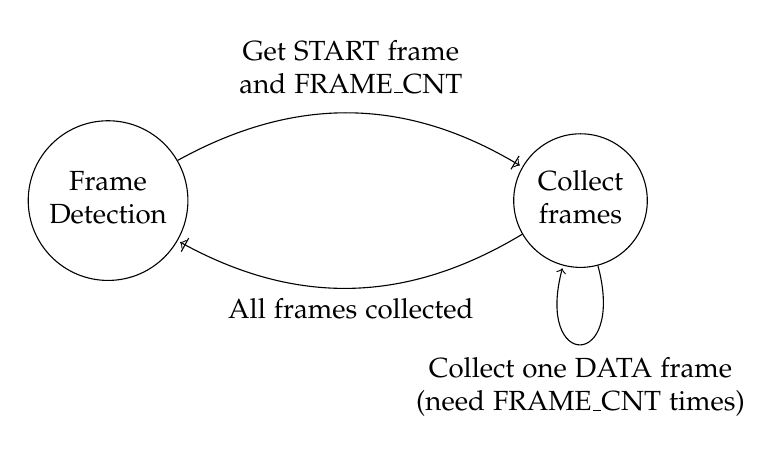
\begin{tikzpicture}[shorten >=1pt,node distance=6cm,on grid,auto]
            \node[state] (q_0)   {\makecell{Frame\\Detection}};
            \node[state] (q_1) [right=of q_0] {\makecell{Collect\\frames}};
            \path[-|>]
            (q_0) edge [bend left] node  {\makecell{Get START frame\\and FRAME\_CNT}} (q_1)
            (q_1) edge [bend left] node  {All frames collected} (q_0)
                edge [loop below] node {\makecell{Collect one DATA frame\\(need FRAME\_CNT times)}} ()
            ;
        \end{tikzpicture}
        }

        \subparagraph{}
        After rebuilding a full packet, the packet is put into the data queue within the MAC object. The packet can then be retrieved back by invoking {\tt recv} function. This function is just a simple call transfer to {\tt Queue.get}. The {\tt recv} function also supports a timeout so that the function can become non-blocking.

    \subsection{Limitation}\label{sec:lim}
    
        \subparagraph{}
        According to the state machine we show above, we now only support to collect one packet at a time. When the state machine start to collect \texttt{DATA} frames according to the last \texttt{START} frame, a new \texttt{START} frame will be \texttt{ACK}ed as if the \texttt{ACK} frame was lost or timed out. By far, the state machine cannot handle two sequence of frames at the same time. This means that we need to ensure the synchronization of sending so that the frames of two packets does not interleave with each other.
        \subparagraph{}
        This problem is discovered when we were writing the tunnel in project 4. For more details, refer to section \ref{sec:ftpsynch}.

\section{Sending}
    \subparagraph{}
    The sending function is a blocking function that can be invoked in any thread. In most cases, this is only invoked by the network layer, but it can still work if the users wants to control the MAC on their own.

    \subsection{Stop and wait}
        \subparagraph{}
        Project 2 requires us to implement a stop-and-wait protocol for sending frames, and the following figure is the state machine for this protocol. This is the default strategy for sending {\tt PING} and {\tt START}.

        \begin{figure}[!h]
	        \centering
	        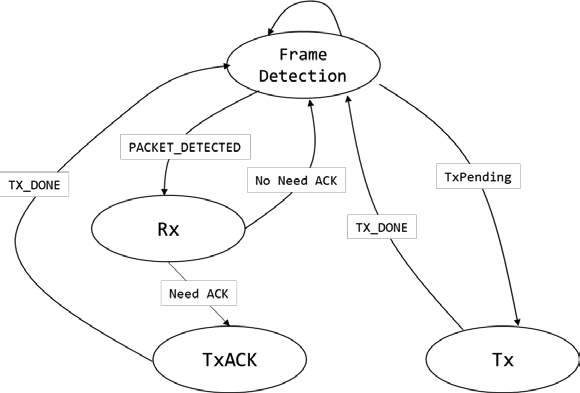
\includegraphics[width=0.5\linewidth]{sections/a.png}
	    \caption{Stop-and-wait state machine}
        \end{figure}
        
        When the MAC gets a frame detected by the physical layer, it first checks if the {\tt DST} field correctly matches the MAC address of itself or if it is a broadcast frame. We denote {\tt 0xff} as the broadcast frame MAC address.

    \subsection{Simple Sliding Window}
        To improve throughput, we added a simple sliding window with fixed window size. Instead of send one frame and wait for one ACK, we send window size of frames in a role and wait for all the ACKs. There could have been one improvement for future work to use the accumulative ACK just like the TCP transmission algorithm. After waiting for a certain amount of time set by the user, the sender checks if there is any frame still not ACKed, and then retransmit them in the next loop. This is the default strategy for sending {\tt DATA} frames.

    \subsection{LT Fountain Encoding}
        When we were handling the network with jamming, we tried to use LT fountain encoding to replace the sliding window algorithm, so that the receiver would not stuck on one frame for a long time. In this strategy, we only send one ACK when the receiver has enough data to recover the whole packet. The sender keeps sending newly generated frame yielded by the encoder and waits for the single ACK. This strategy is disabled by default, but users can enable it on their own.

    \subsection{Priority Queuing}
        To improve the latency of the control frames, including {\tt ACK}, {\tt PING}, {\tt PONG}, we give them a higher priority. The data frames, including {\tt START} and {\tt DATA} has lower priorities. We used the {\tt PriorityQueue} from python library and added the priority tag for each frame to be sent. This ensures that all the control frames, which aims for short latency, to be sent instantly without queuing with the data frames.

    \subsection{Multi-level Random Queue}
        Though priority queue can improve the latency for small control frames, it may block data frame forever when the amount of control frames is too overwhelming. In this case, the throughput of data frames will show great degradation. Thus, we added some pseudo-randomization to ensure the two kinds of frames are transmitted fairly. The chance for transmitting data frames is 25\% and the chance for transmitting control frames is 75\%. Since data frames have relatively large size and control frames have relatively small size, it is acceptable to have a 1:3 chance proportion. This strategy is also disabled by default but users can enable it on their own.

    \subsection{Synchronization}
        As stated in section \ref{sec:lim}, we added a global lock in the MAC object. In the prologue of the data sending function, it acquires the lock. In the epilogue of the data sending function, it releases the lock. The critical section code ensures that no {\tt Exception} would be raised from inside so the lock resource is ensured to be well-managed. For functions that send other frames, including {\tt ACK}, {\tt PING} and {\tt PONG}, we do not need to add the lock, because the frames are queued in the physical layer using python's Queue, which is already atomic by nature.

\section{Carrier Sense Multiple Access}
\subparagraph{}
Carrier Sense Multiple Access(CSMA) request listening the transmission media before send data. Notice in our design of the physical layer, not only we calculate the dot result of the received signal and the template one, but also the power of the former one. Then we can divided the status of the transmission media into three cases:
\begin{itemize}
    \item idle: The power is low
    \item transferring: The power is high, the dot is large
    \item jamming/noise: The power is high, the dot is low
\end{itemize}
Only in the first case we can start a new process of transmission. In the last case that the channel is busy while the content do not match the sending ones, we can judge that there are other nodes using this channel or terrible interfere occurs and we then block the sending thread. After the channel get idle, we execute the back-off strategy and resume the blocked thread(if exists) then the sending function is available again.
\chapter{Network Layer}\label{ch:ch4label}

The network layer adds the IP fields to the packet provided by the transport layer and then give it to the data link layer. In our implementation, this is rather a thin layer since most of the works, including separating large packets has been done by the legacy code in our robust MAC class. Therefore, we only adds the source and destination ip information and just pass the packet to the layer below. As a future work, we may consider move the packet seperation code from the MAC to our IP class.

\section{Packet}
    \subparagraph{}
    We implemented the IPv4 address convention: 4 bytes for source ip address and 4 bytes for destination ip address. The packet structure is as simple as follows. The {\tt PROTOCOL} field can be used by the transport layer, this will be covered in the next chapter.

    $$|PROTOCOL(1B)|SRC\_ADDR(4B)|DST\_ADDR(4B)|PAYLOAD(var)|$$

\section{Static ARP}
    \subparagraph{}
    To send the packet to the correctly destination and also ensure it being correctly recognized by the peer MAC, we need to convert the IP address to the MAC address and send it to the MAC. Since there only exist two hosts in the acoustic network, we assign static IP address without using DHCP. We keeps a python {\tt map} object acting as the ARP table to map the IP address to the corresponding MAC address.

\chapter{Transport Layer}\label{ch:ch5label}

The transport layer provides a network-to-application interface. We call our transport layer Aocket, just like the socket in POSIX. The Aocket object creates a IP object as a member variable. It encapsulates the data given by the applications to ICMP, UDP or TCP and pass to the network layer to transmit to the target peer.

\section{ICMP}
    \subparagraph{}
    The {\tt TYPE} field for ICMP in the IP packet is 1.

    \subsection{Structure}
        \subparagraph{}
        The structure of our ICMP packet is shown below. There {\tt TYPE} field has two types, PING and PONG, with value 0 and 3. They have the same meaning as the standard ICMP packet for echo and echo reply. The {\tt ID} field and {\tt PAYLOAD} field are the same as icmp\_id and pattern in the standard ICMP protocol.

        $$ | TYPE(1B) | ID(1B) | PAYLOAD(var) |$$
        
    The PING packets are automatically replied as PONG packets with the same {\tt ID} and the same {\tt PAYLOAD} in the Aocket.

\section{UDP}
    \subparagraph{}
    UDP is a simple User Datagram Protocol to transmit data between network hosts. Our UDP looks very similar to the standard UDP protocol. The {\tt TYPE} field for UDP in the IP packet is 2.

    \subsection{Structure}
        \subparagraph{}
        The structure of our ICMP packet is shown below. The {\tt SRC\_PORT} and {\tt DST\_PORT} is the same as the standard UDP protocol. The size of the payload can be extracted from the IP packet in the lower layer so we emit that field.
        
        $$| SRC\_PORT(2B) | DST\_PORT(2B) | PAYLOAD(var) |$$
    
    \subsection{Multi-port Connection}\label{sec:mulport}
        \subparagraph{}
        Unlike {\tt socket}, which only supports binding to a single port and stick to only one protocol, our Aocket supports listening to multiple ports with different protocols at the same time. This is because we only have one Aocket instance for the entire Athernet node. However, it helps unlock a lot of potentials of our network. Each open ports has a separate queue to contain the packets we buffer in the Aocket. The sending and receiving operation can be done by specifying the local port in {\tt Aocket.send} and {\tt Aocket.recv}.

\section{Toy TCP}
    \subparagraph{}
    Though we are not required to implement a fully functioning TCP, we still need one protocol to support state transitions of TCP, to support the transmission of FTP packets. Therefore we created a toy TCP that is very similar to the UDP we have, except for a new {\tt FLAG} field. The {\tt TYPE} field for TCP in the IP packet is 3.

    \subsection{Structure}
        \subparagraph{}
        The structure of our toy TCP is shown as follows, it is mostly very similar to the UDP we have. The new {\tt TYPE} field is a subset of TCP flags in the standard TCP specification.
        
        $$| SRC\_PORT(2B) | DEST\_PORT(2B) | TYPE(1B) | PAYLOAD(var) |$$
    
    \subsection{Packet types}
    
        \subparagraph{}
        We have four kinds of TCP packet in our toy TCP: SYN, FIN, DATA and a reserved but not implemented ACK.

        \subparagraph{SYN}
            This flag is for creating a connection between two nodes, which is the same flag in the TCP protocol. This packet can be sent by using {\tt Aocket.connect}. The difference from the TCP standard is that we do not do three-way handshake. The SYN is sent in one way from an Athernet LAN host to another Athernet LAN host. If the destination is indeed a WAN host, the gateway will help do the the handshaking by utilizing {\tt socket}. The {\tt TYPE} field has value 0.
            
        \subparagraph{ACK}
            This flag is only reserved but not implemented. Though we lack the implementation of ACK, the transmission is still reliable between two Athernet nodes since the legacy code in our data link layer ensures the frame can be received correctly. The only problem for lacking ACK is when connecting hosts outside of the Athernet, but on other hand, the gateway uses {\tt socket} to handle ACK automatically, so we do not need to worry too much. The {\tt TYPE} field has value 1.
        
        \subparagraph{FIN}
            This flag is for closing an existing connection between two nodes. This packet can be sent by using {\tt Aocket.close}. Like the SYN in our toy TCP, we do not do four-way handshake. The FIN is also sent from one in one way from an Athernet LAN host to another Athernet LAN host. If the destination is ideed a WAN host, the gateway will help do the four-way handshaking by utilizing {\tt socket} again. The {\tt TYPE} field has value 2.

        \subparagraph{DATA}
            This flag is for transmitting real data between two Athernet LAN nodes. This packet can be sent by using {\tt Aocket.send\_tcp}. This flag is different from the standard TCP protocol because it does not have a explicit DATA flag. When transmitting to a WAN address, the gateway uses {\tt socket.sendto} to forward the content data to the target host. The {\tt TYPE} field has value 3.

    \subsection{Multi-port Connection}
        \subparagraph{}
        Just as mentioned in section \ref{sec:mulport}, the Aocket can also listen to multiple TCP port and send to multiple destinations at the same time.

\chapter{Application: FTP}\label{ch:ch6label}

The application layer protocol we implemented is the File Transfer Protocol (FTP). Since we do not need to implement SSL, we can omit the session layer and the presentation layer and base the FTP client directly on the toy TCP.

\section{Commands}
    \subparagraph{}
    Our FTP client has a interactive command interface, and the user can input the FTP command after each ``{\tt > }'' prompt and see the response from the server after each ``{\tt < }''.
    \subparagraph{}
    We support a subset of FTP commands, USER, PASS, PWD, CWD, PASV, LIST and RETR.  These command represents ``username'', ``password'', ``print working directory'', ``change working directory'', ``passive mode'', ``list directory'' and ``retrieve file''. Our FTP client uses a regular expression to check the validity of the input command, if the command is well-constructed, the command will be directly transmitted to the FTP server and waits for the reply. The client will then check the response FTP code to see if there is an an occurs or the command has performed successfully. In most cases, when an error occur, it won't mess up the FTP client so the client just print out the returned message from the server. When an error message is return during LIST or RETR, the client will cancel the current transmission and return to the.

\section{Multi-port Connection}\label{sec:ftpsynch}
    \subparagraph{}
    After specifying the remote FTP server address and port, the client initiates a toy TCP connection from a local port, as the control stream. The commands are then sent through this connection. When doing LIST or RETR, FTP needs to start a new connection to the destination previously given by the PASV command. Thanks to the multi-port connection feature of our Aocket, our FTP client could initiate a new TCP connection easily. The newly established connection works as the data stream, and data is transmitted from the remote to the local host. When The connection is closed or the transmitted length has reached the file size, the transmitted file or list is stored in a new file the on the local machine. Finally, after the user quit the interactive command interface, the client closes the TCP connection and then quits itself.

\chapter{Cross Layer}\label{ch:ch7label}

This section talks about the cross layer applications we implemented in our project. These applications manipulates both the IP and the transport layer packets, usually used for packet forwarding.

\section{Gateway}

    \subparagraph{}
    The gateway is the only way that connects the Athernet LAN and the WAN, when transmitting from a Athernet LAN host to a remote host, the gateway needs to do some translation jobs to ensure the packet can be correctly recognized by the modern network systems. In addition, the gateway also needs to so it needs to do maintain the NAT table to store the existing connections and exchange of packets in and out the acoustic network.
    
    \subsection{Dynamic Mapping}
        \subparagraph{}
        The dynamic mapping is done by connection, when a packet is received from a Athernet LAN host, the gateway will then check the NAT table if there is a existing connection from the source to the destination. The source is a pair of <source\_ip, source\_port>. If the gateway finds the source in the table, the packet is repacked with the gateway's ip and local port, and the transmit to the remote by using {\tt socket}. If the source does not present in the NAT table, the gateway starts a new connection by creating a new {\tt socket} instance and store it in the NAT table in the entry with key of source.

    \subsection{TCP Connection Forwarding}
        \subparagraph{}
        When the LAN host is sending a TCP packet to the remote host, the gateway needs to convert the packet from our toy TCP packet to the real TCP packet by using {\tt socket}. When receiving a SYN in the toy TCP, the gateway starts a new connection by using the {\tt socket.connect}. When receiving the DATA, the gateway extracts the payload and sends the data via {\tt socket.send}. For the FIN, the gateway just call {\tt socket.close} and then delete the NAT table entry.

    \subsection{Multi-port Listening}
        \subparagraph{}
        As the connections to the WAN peers creates a lot of {\tt socket} connections, we need to use a simple way to collect the ready {\tt socket} streams and transmit the received data back to the Athernet LAN hosts. We created a looping thread that uses the system call ``select'' on the list of all {\tt sockets} objects to retain the ready socket streams, and the put converted Aocket packet back to the sending queue. The only thing special about this thread is the termination of TCP connections. The termination of the transmission is detected by the instant return from {\tt socket.recv} with an empty payload. The thread then sends a FIN back to the Athernet host and deletes the entry in the NAT table.
        
    \subsection{ICMP Endian Issues}
    \subparagraph{}
    There are several problem we met when achieving ICMP. The obvious one is about the endian. We know the standard Ethernet uses big-endian while the common x86 platform runs in little-endian. When we achieve this part, which directly communicates with the exist Ethernet, we have to carefully notice the issues about the endian. Not only the data field but the header information and the checksum are also need to match the correct endian. We once found that the sequence number of the received ICMP Echo Request (PING) is multiplied by 256 for no reason. Then we find out that the corresponding field is 2 bytes and the so called multiplied by 256 is the result of the wrong endian.
    \subparagraph{}
    Another problem is that when the node in the external Internet tries to PING the gateway, the gateway have no idea whether it should reply by self or just pass the request to the nodes in the Intranet. This problem occurs in project3 part5 when we tried to establish a toynet. The way to solve this problem is previously define different patterns in PING request, related to the different node identity in the Intranet and the gateway can determine its behavior due to this pattern. Though we think the solution is not beautiful enough and the gateway in the real world should hide the existence of the internal nodes.

\section{Tunnel}
    \subparagraph{}
    
    The way described in the project requirement sheet says to use the {\tt iptables} utility in Linux command line, but this raise one problem because {\tt iptables} forwarding will drop the destination port information. However, since the destination port is randomly given by the remote server after the PASV command, we do not know which port our data stream should send to in our proxy. Therefore, we choose another common proxy protocol - SOCKS5, which packs the whole IP packet into one TCP packet. By this means, we can forward the packet through our acoustic tunnel correctly to the remote in WAN.

    \subsection{SOCKS5 Proxy}
        \subparagraph{}
        We start a small threaded TCP server by an python class derived from {\tt ThreadingMixIn} and {\tt TCPServer} super classes. The server listens on port 1787 at localhost. After that, we set the FTP client, FileZilla to use the proxy on our local port. Then when a new TCP connection is established, a stream of SOCKS5 packet will be sent to my proxy. We then unpack the SOCKS5 packet and establish a TCP connection using our Athernet and send data through the Aocket. The proxy server runs in a loop so that the data can be exchanged between the SOCKS5 stream and the Aocket. The loop includes two part. One part is by making system call using ``select'' to get data from the local TCP connection stream, and make sure the thread does block but does not block forever. At the same time, we start a simple thread, waiting for the packet from the Aocket and send it to the proxy client.

% \chapter{Auxiliaries}\label{ch:ch8label}

\section{Wave Plotting}

\section{Save and Replay}

% \chapter{Conclusion}\label{ch:conclusion}
In case you have questions, comments, suggestions or have found a bug, please do not hesitate to contact me. You can find my contact details below.
  \begin{center}
    Jesper Kjær Nielsen\\
    \href{mailto: jkn@es.aau.dk}{jkn@es.aau.dk}\\
    \href{http://kom.aau.dk/~jkn}{http://kom.aau.dk/\textasciitilde jkn}\\
    Fredrik Bajers Vej 7\\
    9220 Aalborg Ø
  \end{center}
\printbibliography[heading=bibintoc]
\label{bib:mybiblio}
% \appendix
% \chapter{Appendix A name}\label{ch:appAlabel}
Here is the first appendix
\end{document}